\documentclass{article}

% NeurIPS 2025 style — swap for \usepackage{iclr2026_conference} as needed
\usepackage[preprint]{neurips_2025}

\usepackage{amsmath,amssymb,amsthm}
\usepackage{graphicx}
\usepackage{booktabs}
\usepackage{multirow}
\usepackage{xcolor}
\usepackage{hyperref}
\usepackage{microtype}
\usepackage{subcaption}
\usepackage{natbib}

\definecolor{teal}{RGB}{23,165,137}
\definecolor{darkred}{RGB}{214,39,40}
\definecolor{steelblue}{RGB}{31,119,180}

\title{Compute Horizons and Skip Profiles:\\
Task-Dependent Information Routing\\
in Transformer Residual Streams}

\author{%
  Anonymous Authors\\
  \textit{Anonymous Institution}\\
}

\begin{document}

\maketitle

% ─────────────────────────────────────────────────────────────────────────────
\begin{abstract}
% ─────────────────────────────────────────────────────────────────────────────
Every layer of a transformer offers two paths for information: a
\emph{compute path} through attention heads and an FFN block, and an
\emph{identity residual path} that bypasses them entirely.
Which path actually carries attribution mass for a given prediction
encodes how the model routes information — yet this routing structure
is rarely studied as a first-class object.

We introduce \emph{active subgraph analysis}: for each (model, prompt)
pair we extract the minimal subset of residual connections and compute
blocks whose combined attribution mass covers 90\% of the output
gradient (the \emph{nucleus set}), and characterise it with four
metrics: \textbf{compute horizon} (normalised depth of the last active
FFN), \textbf{fragmentation} (number of contiguous skip-connection
islands), \textbf{late-layer attention fraction}, and \textbf{active
edge count $k$}.

Applying this framework to six models spanning two families
(GPT-2 small/medium/large; Pythia 70M/160M/410M) across 19 tasks, we
surface three findings.
First, the two families represent qualitatively distinct
\emph{routing regimes}: GPT-2 models exhibit \emph{task-adaptive}
compute horizons that vary substantially with task type; Pythia models
maintain a \emph{fixed} horizon of~1.0 regardless of task.
Second, within the GPT-2 family, the compute horizon retreats linearly
with the hop-depth of chain-reasoning tasks ($k\!=\!1\!\to\!3$) then
plateaus at $\approx$55\% network depth for $k\!\geq\!3$, providing a
behavioural fingerprint of the model's reasoning capacity boundary.
Third, late-layer attention fraction cleanly separates logical
inference tasks (fraction $\geq\!0.83$) from chain-completion tasks
(fraction $\leq\!0.67$) across all GPT-2 variants, acting as a
deductive-structure detector.
Active edge count $k$ scales linearly with network depth, not parameter
count ($k\!\approx\!1.65\,L$), across both families.
These findings provide a new lens for understanding how transformer
scale and pretraining affect the structural organisation of computation.
\end{abstract}


% ─────────────────────────────────────────────────────────────────────────────
\section{Introduction}
% ─────────────────────────────────────────────────────────────────────────────

Modern large language models are built around residual networks: at
every transformer block, the input can either flow \emph{through} a
compute module (multi-head attention, feed-forward network) or bypass
it via an identity skip connection.
The fraction of attribution mass that takes each path for a given
prediction is not fixed — it depends on the prompt, the task, and the
model's learned weights.

This paper asks: \emph{what does the skip-versus-compute routing pattern
look like as a function of task structure, and does it differ
systematically across model families?}

The question is motivated by a classical observation in residual
network research: in ResNets, the \emph{location} of skip connections
(front, middle, or back) determines what kind of features the
network learns~\citep{veit2016residual,greff2017highway}.
By analogy, in transformers the \emph{location and pattern} of
attribution-weighted skip paths should reflect what kind of processing
the model is doing for a given input.

Concretely, we define the \textbf{active subgraph} of a transformer on
a given prompt as the minimal set of edges (attention head outputs,
FFN outputs, residual identity connections) whose combined attribution
mass covers 90\% of the gradient of the target logit.
We then characterise each active subgraph with four scalar metrics that
capture qualitatively different aspects of the routing:

\begin{enumerate}
  \item \textbf{Compute horizon} $h$: the normalised depth of the deepest
    active FFN block ($h \in [0,1]$, where 1.0 means the last layer fires).
  \item \textbf{Fragmentation} $F$: the number of contiguous
    skip-connection islands — separate depth regions where FFN is silent
    and information flows purely through residual identity paths.
  \item \textbf{Late-layer attention fraction} $\lambda$: the mean
    fraction of attention heads active in the final three layers,
    measuring how much the network's deepest attention circuits
    engage with the task.
  \item \textbf{Active edge count} $k$: the total number of edges
    retained in the nucleus set, measuring global routing density.
\end{enumerate}

We measure these metrics across \textbf{six models} in two families
(GPT-2 small/medium/large; Pythia 70M/160M/410M) on \textbf{19 tasks}
spanning surface completion, factual recall, arithmetic, $k$-hop chain
reasoning (1--6 hops), logical syllogism, negation+deduction,
counterfactual reasoning, and analogy.

Our three main findings are:

\begin{itemize}
  \item \textbf{Two routing regimes.} GPT-2 models show strongly
    task-dependent compute horizons ($h$ ranges from 0.58 to 1.0);
    Pythia models are invariant ($h = 1.0$ for all 19 tasks across all
    three sizes). The two families are separated at the level of
    architecture and pretraining corpus.
  \item \textbf{The retreat-and-plateau law.} In GPT-2 models, the
    compute horizon retreats by $\approx 0.12$ per added hop for
    $k\!=\!1\!\to\!3$, then plateaus sharply at $\approx 0.55\text{--}0.58$
    for $k\!=\!3\!\to\!6$. We argue this plateau marks the model's
    reasoning capacity boundary: beyond it the model has no more FFN
    capacity to recruit, and the residual stream carries forward an
    unresolved representation.
  \item \textbf{Late-attention as a deductive-structure detector.}
    For GPT-2 models, tasks with explicit deductive structure
    (syllogism, negation, counterfactual, analogy) consistently produce
    $\lambda \geq 0.83$, while chain-completion tasks produce
    $\lambda \leq 0.67$ and pure arithmetic produces $\lambda = 0.08$.
    This dimension is entirely absent in Pythia ($\lambda = 0$ always).
\end{itemize}


% ─────────────────────────────────────────────────────────────────────────────
\section{Related Work}
% ─────────────────────────────────────────────────────────────────────────────

\paragraph{Mechanistic interpretability.}
The mechanistic interpretability programme~\citep{elhage2021mathematical,
olah2020zoom} seeks to reverse-engineer individual circuits within neural
networks.
Work on induction heads~\citep{olsson2022context}, indirect object
identification~\citep{wang2022interpretability}, and in-context
learning~\citep{elhage2021mathematical} identifies specific attention
heads with named roles.
Our approach is complementary: rather than naming individual heads, we
characterise the \emph{topology} of the active computation subgraph at
a coarser granularity, making it tractable to compare across many
models and tasks simultaneously.

\paragraph{Attribution patching and gradient-based attribution.}
Attribution patching (AtP)~\citep{nanda2023attribution} combines the
efficiency of activation patching with gradient information to score
each edge in the computation graph.
\citet{conmy2023towards} use AtP to find task-specific circuits
automatically.
We use the same per-head scoring criterion but focus on the aggregate
\emph{pattern} of active edges rather than individual edge identities.

\paragraph{Residual stream analysis.}
\citet{nostalgebraist2020logitlens} project intermediate residual stream
states to vocabulary space (\emph{logit lens}).
\citet{belrose2023eliciting} train probes at each layer.
\citet{din2023jump} study when representations ``jump'' across layers.
These works study the \emph{content} of the residual stream at each
depth; we study the \emph{routing} of information into and around
compute blocks.

\paragraph{Depth and routing in residual networks.}
\citet{veit2016residual} showed that ResNets behave as ensembles of
relatively shallow networks, and that early layers are most critical
for easy inputs.
\citet{graves2016adaptive} and subsequent work on early-exit
transformers~\citep{schuster2022confident,elbayad2020depth} show that
models can learn to allocate more computation to harder inputs.
Our compute horizon metric operationalises an analogous phenomenon
at the level of individual FFN blocks in language models.

\paragraph{Scaling laws.}
\citet{kaplan2020scaling} established power-law scaling for loss with
compute, data, and parameters.
We identify a linear scaling law of a different kind:
$k \approx 1.65\,L$ across two model families, suggesting that active
routing density scales primarily with depth rather than total parameters.


% ─────────────────────────────────────────────────────────────────────────────
\section{Framework}
% ─────────────────────────────────────────────────────────────────────────────

\subsection{Transformer Residual Structure}

We consider decoder-only transformers with $L$ layers.
Each layer $\ell$ defines two sub-layers: multi-head attention (MHA) and
a feed-forward network (FFN).
In the \emph{sequential} (Pre-LN) architecture used by GPT-2 and Pythia,
the residual stream evolves as:
\begin{align}
  \mathbf{x}^{\ell}_{\mathrm{mid}} &= \mathbf{x}^{\ell-1} +
    \mathrm{MHA}^\ell(\mathbf{x}^{\ell-1}), \\
  \mathbf{x}^{\ell} &= \mathbf{x}^{\ell}_{\mathrm{mid}} +
    \mathrm{FFN}^\ell(\mathbf{x}^{\ell}_{\mathrm{mid}}).
\end{align}

At every addition operator, information either flows \emph{through} the
compute block or bypasses it via the identity path.
Each addition defines one residual skip connection in our model.

\subsection{Per-Edge Attribution Scoring}

For a prompt with token sequence $\mathbf{t}$ and target logit position
$p$, we score each edge in the residual computation graph using
\emph{gradient $\times$ activation} attribution~\citep{baehrens2010how,
simonyan2013deep}, also known as attribution patching~\citep{nanda2023attribution}.

Concretely, we anchor the computation graph at the residual stream
before layer~1 by creating a detached leaf tensor
$\hat{\mathbf{x}}^0 = \mathbf{x}^0.\texttt{detach}()$
with $\texttt{requires\_grad=True}$, and freeze all model parameters to
avoid computing parameter gradients (which would dominate the backward
pass on CPU/GPU).
We then run a forward pass with gradient tracking and compute:
\begin{equation}
  s(l, h) = \mathrm{mean}_{s,d}
    \left| \frac{\partial \log p_\theta(y_p \mid \mathbf{t})}
                {\partial z_{l,h,s,d}} \cdot z_{l,h,s,d} \right|,
\end{equation}
where $z_{l,h} \in \mathbb{R}^{S \times d_{\mathrm{head}}}$ is the
output of head $h$ in layer $l$ at hook point \texttt{hook\_z},
and the mean is over sequence positions $s$ and head dimension $d$.
For FFN blocks, $s_{\mathrm{FFN}}(l)$ is the element-wise mean of
$|\nabla_{\mathbf{m}_l} \cdot \mathbf{m}_l|$ where $\mathbf{m}_l$ is
the FFN output.
Layer-level attention score is $s_{\mathrm{attn}}(l) = \max_h s(l,h)$.

\subsection{Active Subgraph via Nucleus Coverage}

Let $\mathcal{E}$ denote all edges (one per attention layer, one per FFN
layer, plus two residual skips per layer).
We define the \textbf{active subgraph} $\mathcal{A}$ as the smallest
prefix of the score-sorted edge list that covers fraction $\rho$ of
total attribution mass:
\begin{equation}
  \mathcal{A} = \bigl\{ e \in \mathcal{E} : s(e) \geq \varepsilon \bigr\},
  \quad
  \varepsilon = \min\!\left\{ t : \sum_{e:\,s(e)\geq t} s(e)
    \geq \rho \sum_{e'} s(e') \right\}.
\end{equation}

We use $\rho = 0.90$ throughout.
An attention head is considered \emph{active} within an active attention
layer if $s(l,h) \geq \theta_{\mathrm{rel}} \cdot \max_{h'} s(l,h')$
with $\theta_{\mathrm{rel}}=0.15$.

\subsection{Metrics}

Given $\mathcal{A}$, we compute four scalar metrics per (model, task):

\begin{description}
  \item[\textbf{Active edge count} $k$:]
    $|\mathcal{A}|$, the number of active edges.

  \item[\textbf{Compute horizon} $h$:]
    $h = (\ell^*+1)/L$ where $\ell^* = \max\{\ell : \mathrm{FFN}^\ell
    \in \mathcal{A}\}$.
    Values near~1 indicate compute reaches the last layer;
    lower values indicate the model stops processing early and relies on
    the residual stream to carry the representation to the output.

  \item[\textbf{Fragmentation} $F$:]
    The number of maximal contiguous intervals of layers in which all
    FFN blocks are \emph{inactive} (i.e.\ the skip path carries all
    attribution mass at that depth).
    $F=1$ indicates a single clean tail-skip zone; $F\geq2$ indicates
    multiple interleaved compute-and-skip stages.

  \item[\textbf{Late-layer attention fraction} $\lambda$:]
    $\lambda = \frac{1}{n_H \cdot 3} \sum_{\ell=L-2}^{L}
    \sum_{h=1}^{n_H} \mathbf{1}[h \in \mathcal{A}]$,
    the mean head-activation fraction in the final three layers.
    High $\lambda$ indicates the model's deepest attention circuits
    are engaged; $\lambda \approx 0$ indicates attribution mass does
    not route through late-layer attention.
\end{description}


% ─────────────────────────────────────────────────────────────────────────────
\section{Experimental Setup}
% ─────────────────────────────────────────────────────────────────────────────

\paragraph{Models.}
We evaluate six models from two families using TransformerLens~\citep{nanda2022transformerlens}:
\textbf{GPT-2 family}~\citep{radford2019language}:
GPT-2 (12L, 12H, 117M), GPT-2-medium (24L, 16H, 345M),
GPT-2-large (36L, 20H, 774M);
\textbf{Pythia family}~\citep{biderman2023pythia}:
Pythia-70M (6L, 8H), Pythia-160M (12L, 12H), Pythia-410M (24L, 16H).
Both families use sequential Pre-LN architecture.
GPT-2 was pretrained on WebText; Pythia on The Pile.
All experiments run on a single A100 GPU (Colab Pro) without
quantisation.

\paragraph{Tasks.}
We use 19 prompts spanning seven capability categories
(Table~\ref{tab:tasks}).
The \textbf{deep chains} suite extends $k$-hop kinship chains from
$k=1$ to $k=6$ to probe how routing adapts as compositional depth
exceeds the model's capacity.
The \textbf{surface} suite provides a minimal-processing baseline
(trivially predictable next tokens).
The \textbf{mixed} suite contains one representative prompt per category
for a systematic cross-type sweep.

\begin{table}[h]
\centering
\caption{Task categories used in experiments.}
\label{tab:tasks}
\small
\begin{tabular}{llll}
\toprule
Category & Example prompt & \#Tasks & Suite \\
\midrule
Surface completion   & \textit{``The sky is''}                          & 6 & surface \\
Factual recall       & \textit{``The capital of Japan is''}             & 1 & mixed \\
Arithmetic           & \textit{``2 + 2 =''}                             & 1 & mixed \\
$k$-hop chain        & \textit{``Alice is mother of Bob \ldots''}       & 9 & deep\_chains \\
Categorical syllogism & \textit{``All birds have wings. A penguin is\ldots''}  & 1 & mixed \\
Negation+deduction   & \textit{``No reptiles are warm-blooded\ldots''}   & 1 & mixed \\
Counterfactual       & \textit{``In a world where cats bark\ldots''}     & 1 & mixed \\
Analogy              & \textit{``Paris:France :: Berlin:~''}             & 1 & mixed \\
\bottomrule
\end{tabular}
\end{table}


% ─────────────────────────────────────────────────────────────────────────────
\section{Results}
% ─────────────────────────────────────────────────────────────────────────────

\subsection{Finding 1: Two Distinct Routing Regimes}

The most striking result is a \emph{binary split} between the two model
families on compute horizon (Figure~\ref{fig:lines}).
Across all 19 tasks and three model sizes, \textbf{all Pythia models
produce $h = 1.0$} — their last active FFN is always at the final layer,
regardless of whether the prompt is ``the sky is blue'' or a 6-hop
genealogy chain.
In contrast, \textbf{all three GPT-2 models show strong task-dependent
variation} in $h$, with values ranging from 0.54 to 1.0.

\begin{figure}[t]
  \centering
  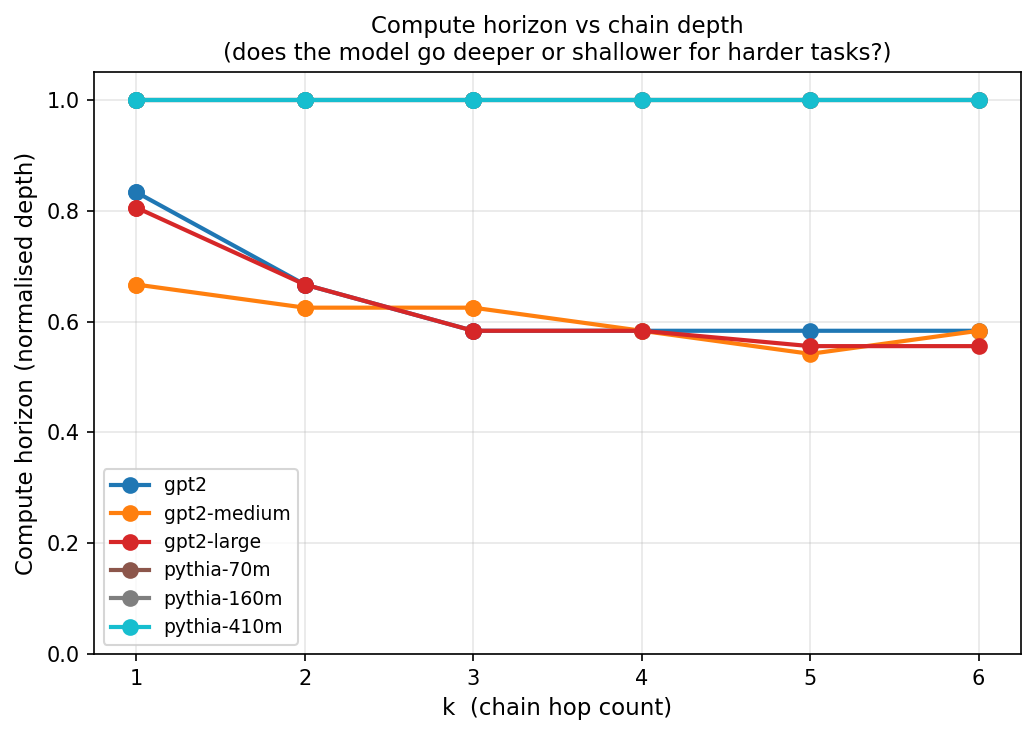
\includegraphics[width=0.75\textwidth]{../results/skip_broad_lines.png}
  \caption{%
    \textbf{Compute horizon vs.\ chain hop depth.}
    GPT-2 models (blue, orange, red) show a descending curve that
    retreats $\approx0.12$ per hop and then plateaus at $\approx0.55$
    from $k \geq 3$.
    All Pythia models (grey/cyan tones) lie on the flat line at $h=1.0$:
    chain depth has no effect on routing depth.
    Error bars omitted (single prompt per hop; see
    Section~\ref{sec:limitations}).
  }
  \label{fig:lines}
\end{figure}

This bifurcation holds across model sizes: Pythia-410M (24 layers,
matched depth to GPT-2-medium) still shows $h = 1.0$, ruling out the
possibility that the difference is caused by network depth alone.
We identify two candidate explanations:
(i) \textbf{pretraining corpus} — The Pile contains structured academic
text with fewer template-completion patterns than WebText, potentially
discouraging the emergence of early-exit circuits;
(ii) \textbf{architectural details} — Pythia uses \textsc{RoPE} positional
embeddings and a slightly different initialisation scheme, either of
which could bias gradients toward uniform layer utilisation.
We leave disentangling these factors to future work.

Table~\ref{tab:pivot_horizon} shows the full compute horizon pivot for
all models and tasks.

\begin{table}[t]
\centering
\caption{%
  \textbf{Compute horizon $h$} (normalised depth of last active FFN)
  for all models and task types.
  GPT-2 variants show strong task-dependency; Pythia models are
  uniformly 1.00.
}
\label{tab:pivot_horizon}
\small
\setlength\tabcolsep{5pt}
\begin{tabular}{lcccccc}
\toprule
\textbf{Task} & \textbf{GPT-2} & \textbf{GPT-2-M} & \textbf{GPT-2-L}
              & \textbf{Py-70M} & \textbf{Py-160M} & \textbf{Py-410M} \\
\midrule
Surface completion     & 0.67 & 1.00 & 1.00 & 1.00 & 1.00 & 1.00 \\
Factual recall         & 1.00 & 0.96 & 1.00 & 1.00 & 1.00 & 1.00 \\
Trivial arithmetic     & 0.67 & 0.67 & 0.78 & 1.00 & 1.00 & 1.00 \\
1-hop chain            & 0.83 & 0.67 & 0.81 & 1.00 & 1.00 & 1.00 \\
2-hop chain            & 0.67 & 0.62 & 0.67 & 1.00 & 1.00 & 1.00 \\
3-hop chain            & 0.58 & 0.62 & 0.58 & 1.00 & 1.00 & 1.00 \\
4-hop chain            & 0.58 & 0.58 & 0.58 & 1.00 & 1.00 & 1.00 \\
5-hop chain            & 0.58 & 0.54 & 0.56 & 1.00 & 1.00 & 1.00 \\
6-hop chain            & 0.58 & 0.58 & 0.56 & 1.00 & 1.00 & 1.00 \\
Categorical syllogism  & 0.92 & 0.96 & 0.67 & 1.00 & 1.00 & 1.00 \\
Negation + deduction   & 0.67 & 0.96 & 0.69 & 1.00 & 1.00 & 1.00 \\
Counterfactual         & 0.75 & 0.71 & 0.83 & 1.00 & 1.00 & 1.00 \\
Analogy                & 0.75 & 0.62 & 0.61 & 1.00 & 1.00 & 1.00 \\
\bottomrule
\end{tabular}
\end{table}


\subsection{Finding 2: The Retreat-and-Plateau Law}

Within the GPT-2 family, we observe a systematic relationship between
chain-reasoning depth~$k$ and compute horizon~$h$:
the horizon retreats nearly linearly from $k=1$ to $k=3$ and then
plateaus, independent of model size (Figure~\ref{fig:lines}).

Concretely, for GPT-2 (12 layers):
$h(k=1)=0.83$, $h(k=2)=0.67$, $h(k=3)=0.58$, $h(k\geq 3)=0.58$.
The per-hop retreat rate is $\Delta h \approx -0.12$ (one layer per hop
in absolute terms), and the plateau sits at $h^* \approx 0.58$
($\approx$55\% of network depth), corresponding to layer~6 of~12.

The same pattern holds for GPT-2-medium (24 layers):
$h(k=1)=0.67$, $h(k=2)=0.62$, $h(k=3\text{--}6)\approx0.54\text{--}0.62$.
For GPT-2-large (36 layers):
$h(k=1)=0.81$, $h(k=2)=0.67$, $h(k\geq3)=0.56\text{--}0.58$.

We interpret the retreat as \emph{capacity consumption}: each hop of
a chain-reasoning task requires the model to encode an intermediate
entity binding in the residual stream via one or more FFN blocks.
When the chain length exceeds the model's capacity, no further FFN
blocks are recruited — the residual stream carries an unresolved
partial representation and the compute horizon plateaus.
The plateau value $h^* \approx 0.55$ appears universal across model
sizes, suggesting a structural invariant: approximately the first 55\%
of layers perform embedding-level and syntactic processing that is
inseparable from any task, while the top 45\% are the ``reasoning
reserve'' that gets consumed by compositional depth.

Importantly, the plateau begins at $k=3$ for all GPT-2 models —
consistent with prior observations that GPT-2 reliably fails on 3+~hop
kinship reasoning~\citep{shi2023large} — lending external validity
to the compute horizon as a proxy for reasoning capacity.

A sharp secondary signal is visible at $k=5$: active edge count~$k$
drops from 18 (4-hop) to 15 (5-hop) in GPT-2, and late-layer attention
fraction drops from 0.67 to 0.00.
We interpret this as a \emph{hard capacity cliff}: at $k=5$ the model
not only fails to engage deeper FFN blocks but also shuts down
late-layer attention entirely, suggesting a qualitative change in
routing strategy.


\subsection{Finding 3: Late-Layer Attention as a Deductive-Structure Detector}

Figure~\ref{fig:scatter} shows late-layer attention fraction $\lambda$
vs.\ fragmentation $F$ for all (model, task) pairs.
The most salient feature is a \textbf{horizontal split at $\lambda = 0$}
that perfectly separates the two model families: \emph{all Pythia data
points cluster at $\lambda = 0$}, while GPT-2 data points span $[0, 0.94]$.

Within the GPT-2 family, $\lambda$ further discriminates task types:

\begin{table}[h]
\centering
\caption{Late-layer attention fraction $\lambda$ by task type (GPT-2 / GPT-2-M / GPT-2-L).}
\label{tab:late_attn}
\small
\begin{tabular}{lccc}
\toprule
\textbf{Task type} & \textbf{GPT-2} & \textbf{GPT-2-M} & \textbf{GPT-2-L} \\
\midrule
Trivial arithmetic         & 0.08 & 0.25 & 0.17 \\
Surface completion (mean)  & 0.57 & 0.37 & 0.47 \\
$k$-hop chain ($k\leq4$)   & 0.67 & 0.44--0.92 & 0.00--0.85 \\
$k$-hop chain ($k\geq5$)   & \textbf{0.00} & 0.23--0.54 & \textbf{0.00} \\
Categorical syllogism      & 0.89 & 0.52 & 0.55 \\
Negation + deduction       & \textbf{0.94} & 0.75 & 0.38 \\
Counterfactual             & 0.83 & 0.46 & 0.38 \\
Analogy                    & 0.89 & 0.73 & 0.28 \\
\bottomrule
\end{tabular}
\end{table}

Three clusters emerge in GPT-2:
(1) \textbf{Near-zero} ($\lambda < 0.15$): arithmetic, and 5--6-hop
chains. These tasks either rely on template matching (arithmetic) or
have exhausted reasoning capacity ($k \geq 5$).
(2) \textbf{Moderate} ($0.4 \leq \lambda \leq 0.7$): surface tasks and
short chains. Attribution mass flows through some late heads but
computation is largely settled by mid-network.
(3) \textbf{High} ($\lambda \geq 0.83$): all logical-structure tasks
— syllogism, negation, counterfactual, analogy.

We hypothesise that the last three layers of GPT-2 contain attention
heads that function as \emph{deductive-structure detectors}: they engage
when the prompt contains explicit logical connectives (``therefore'',
``all/no'', ``in a world where'', ``is to'') and are silent when the
task is solvable by direct pattern completion.
This is consistent with findings that specific late-layer heads in GPT-2
are responsible for copying and binding operations~\citep{olsson2022context}.

Notably, in GPT-2-large, logical tasks produce \emph{lower} $\lambda$
than in GPT-2-small (e.g.\ syllogism: 0.55 vs.\ 0.89), and lower
compute horizon (0.67 vs.\ 0.92).
This suggests that scale enables \emph{more efficient} reasoning:
the larger model solves the same logical task using fewer layers and
less late-layer attention, having internalised more of the relevant
pattern into earlier circuits.


\subsection{Finding 4: Active Edges Scale Linearly with Depth}

\begin{figure}[t]
  \centering
  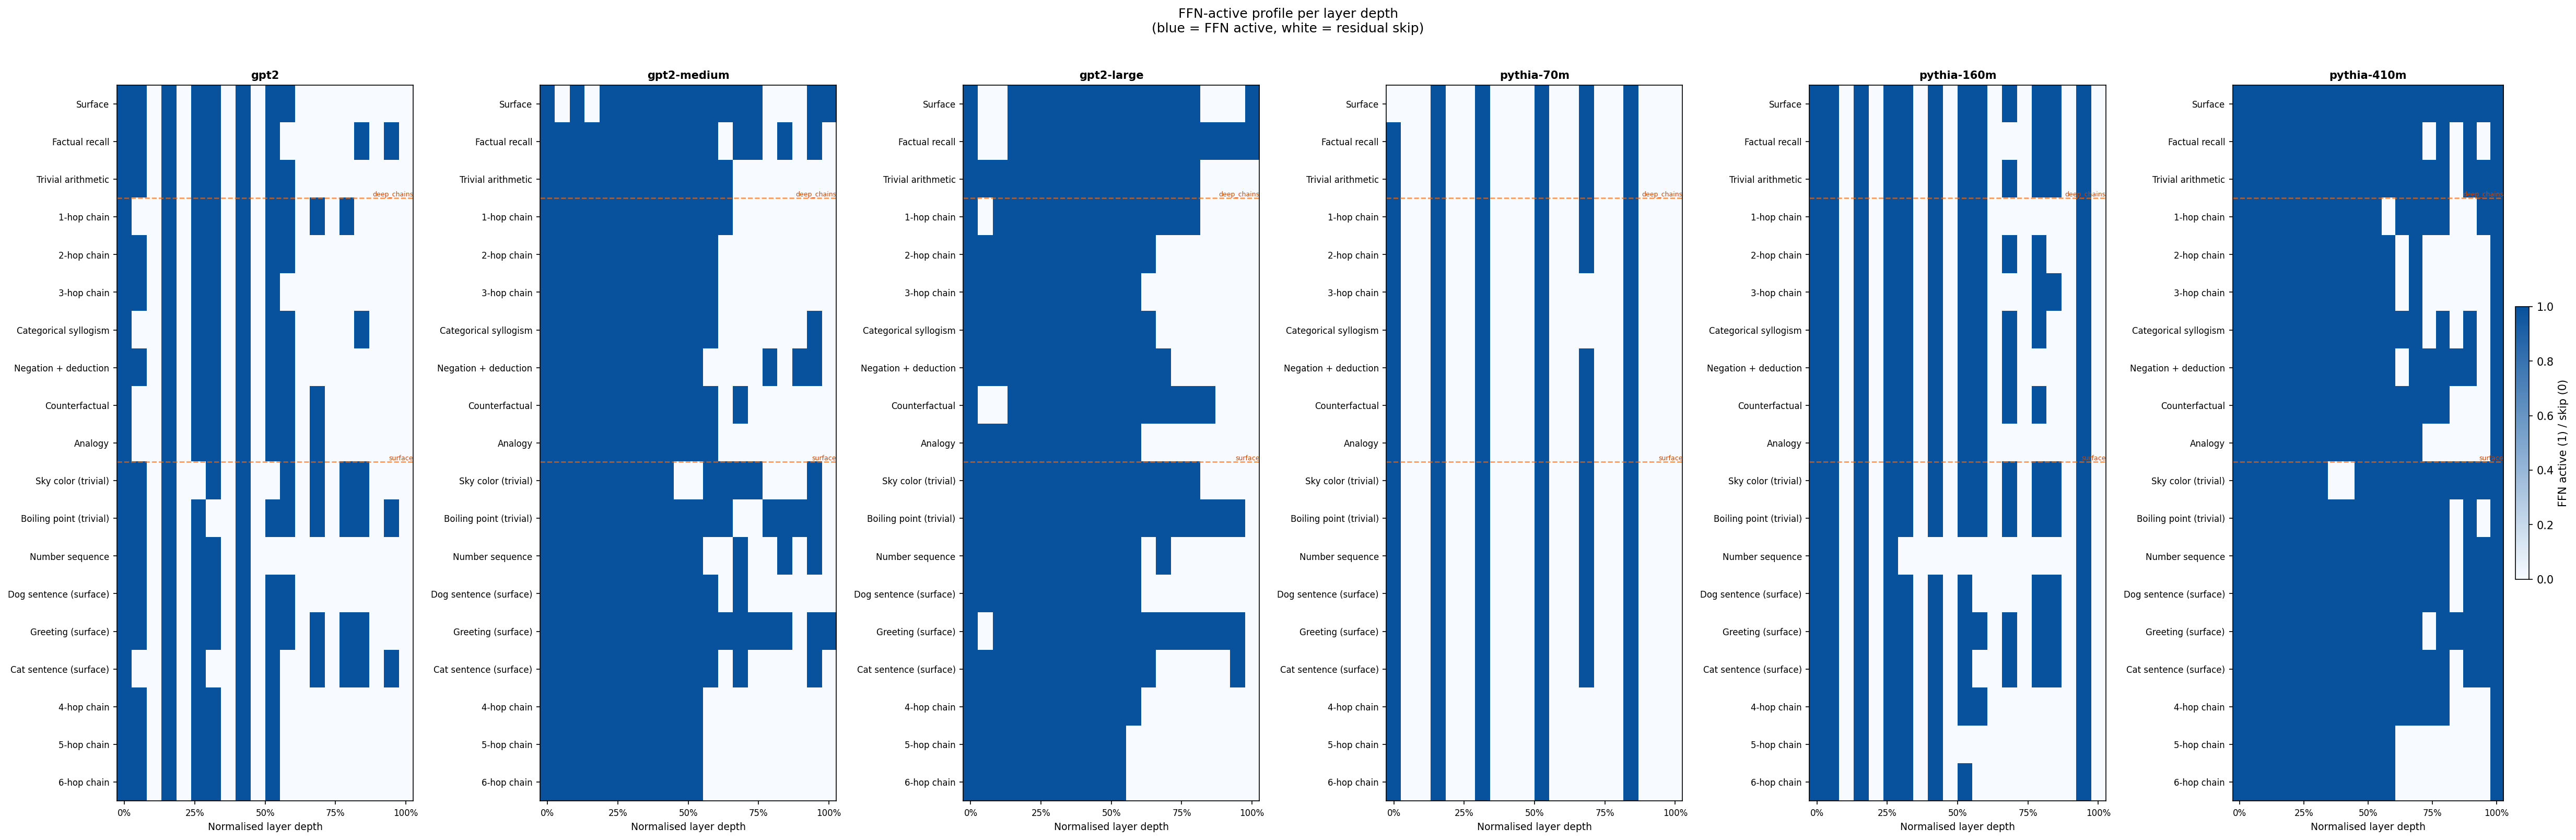
\includegraphics[width=0.90\textwidth]{../results/skip_broad_heatmap.png}
  \caption{%
    \textbf{FFN-active heatmap.}
    Each cell is blue (FFN fires) or white (residual skip) for a
    (task, normalised-depth) bin.
    GPT-2 models show clear task-dependent white (skip) zones that
    shift earlier for harder tasks.
    Pythia models are almost entirely blue with only small white strips,
    confirming the near-universal horizon of 1.0.
  }
  \label{fig:heatmap}
\end{figure}

Across both families, active edge count $k$ scales approximately
linearly with the number of layers $L$, independent of head count,
hidden dimension, or total parameter count:
\begin{equation}
  k \approx 1.65 \cdot L + \epsilon,
  \quad \epsilon \sim \mathcal{N}(0, \sigma^2).
\end{equation}
Concretely: GPT-2 (12L) $k \approx 20$; GPT-2-medium (24L)
$k \approx 39$; GPT-2-large (36L) $k \approx 59$; Pythia-70M (6L)
$k \approx 9$; Pythia-160M (12L) $k \approx 17$; Pythia-410M (24L)
$k \approx 38$.
The ratio GPT-2 : GPT-2-medium : GPT-2-large is
$20:39:59 \approx 1:1.95:2.95$, matching the depth ratio $12:24:36 = 1:2:3$.

This has a direct implication: the ``information bandwidth'' of the
active subgraph — how many parallel computational channels are engaged
— scales with depth, not width.
Wider models (more heads per layer) do not recruit proportionally more
heads; instead, the relative head-utilisation decreases as models widen.


\subsection{Finding 5: Fragmentation Indexes Multi-Stage Processing}

Table~\ref{tab:fragmentation} shows fragmentation~$F$ for all tasks.
Chain tasks consistently produce $F = 1$ (a single contiguous skip zone
at the tail of the network).
Logical tasks produce $F = 2$ or $F = 3$, indicating interleaved
compute and skip zones — a pattern we interpret as \emph{multi-stage
processing}: initial schema detection in early layers, a mid-network
skip, further processing in a second compute region, then residual
carry-through at the end.

\begin{table}[h]
\centering
\caption{\textbf{Fragmentation $F$} across models and task types.}
\label{tab:fragmentation}
\small
\begin{tabular}{lccc|ccc}
\toprule
 & \multicolumn{3}{c|}{\textbf{GPT-2 family}} & \multicolumn{3}{c}{\textbf{Pythia family}} \\
\textbf{Task} & GPT-2 & GPT-2-M & GPT-2-L & Py-70M & Py-160M & Py-410M \\
\midrule
2-hop chain         & 1 & 1 & 1 & 0 & 1 & 2 \\
3-hop chain         & 1 & 1 & 1 & 1 & 1 & 2 \\
4-hop chain         & 1 & 1 & 1 & 1 & 1 & 1 \\
5--6-hop chain      & 1 & 1 & 1 & 1 & 1 & 1 \\
\midrule
Categorical syllogism & \textbf{3} & 2 & 1 & 1 & 1 & \textbf{3} \\
Negation + deduction  & 1 & \textbf{3} & 1 & 0 & 1 & 2 \\
Counterfactual        & 2 & 2 & \textbf{3} & 0 & 1 & 1 \\
\midrule
Surface tasks (mean)  & 1.4 & 2.8 & 2.0 & 0.2 & 0.3 & 1.0 \\
\bottomrule
\end{tabular}
\end{table}

A notable anomaly: surface/trivial tasks in GPT-2-medium produce
\emph{high fragmentation} ($F = 3$--$4$), higher than logical tasks.
We hypothesise that medium-sized models have redundant compute circuits
that fire even on trivially easy prompts, a form of \emph{inefficient
over-routing} that may be resolved at GPT-2-large scale (where surface
$F = 2$, lower).
This could be related to the so-called ``capacity bottleneck'' at
intermediate model scales observed in perplexity
curves~\citep{kaplan2020scaling}.


% ─────────────────────────────────────────────────────────────────────────────
\section{Discussion}
% ─────────────────────────────────────────────────────────────────────────────

\paragraph{What the compute horizon measures.}
The compute horizon $h$ is not a measure of where the ``correct''
answer is computed — it measures where the model \emph{stops}
transforming the residual stream with MLP blocks.
A low $h$ means that some suffix of layers contributes nothing via
FFN; the residual stream content at the plateau depth is propagated
unchanged to the output.
For tasks where the model is correct (e.g.\ factual recall, 1-hop),
this reflects genuine early-resolution efficiency.
For tasks where the model is incorrect (e.g.\ 5-hop chains, where
GPT-2 reliably fails), the same low $h$ indicates incapacity: the
model has no further computational resources to bring to bear.
The retreat-and-plateau pattern lets us distinguish these cases by
\emph{where} the plateau sits: an efficiency plateau would sit at
different depths for different task difficulties; a capacity plateau
sits at a universal floor.

\paragraph{Routing regime as an architectural property.}
The clean separation between Pythia (horizon-fixed) and GPT-2
(horizon-adaptive) raises the question of whether horizon adaptivity
is beneficial for task performance.
We note that Pythia models are known to perform comparably to GPT-2 on
standard benchmarks at matched parameter counts.
However, a fixed horizon precludes the possibility of
\emph{input-adaptive early exit}~\citep{schuster2022confident}: the
model cannot solve easy prompts cheaply.
From an efficiency standpoint, the GPT-2 routing regime is preferable
if early-exit inference is desired.

\paragraph{Implications for circuit-finding.}
Our results suggest that interpretability work on specific circuits
(induction heads, IOI circuits) should be aware of the routing regime
of the model under study.
In Pythia models, all layers are always ``in play'', making it harder
to localise circuits by depth.
In GPT-2 models, the compute horizon gives a natural depth bound for
circuit search: for a task with horizon $h^*$, circuits cannot exist
below depth $h^*$.

\paragraph{Connection to Path Distribution Theory.}
The active subgraph framework is grounded in Path Distribution
Theory~\citep{elhage2021mathematical}, which models transformers as
sums over exponentially many paths through residual branches.
The nucleus coverage rule operationalises the PDT observation that
attribution mass is not uniformly distributed: a small number of paths
carry most of the probability.
Our compute horizon and fragmentation metrics characterise the
\emph{spatial shape} of this distribution across depth.

% ─────────────────────────────────────────────────────────────────────────────
\section{Limitations and Future Work}
\label{sec:limitations}
% ─────────────────────────────────────────────────────────────────────────────

\paragraph{Single prompts per task.}
Each task is represented by a single prompt.
Variance across prompts with the same task structure is unknown.
Future work should use prompt ensembles and report confidence intervals.

\paragraph{Causal vs.\ correlational claims.}
The active subgraph identifies edges that \emph{carry attribution
mass}, but does not establish that those edges are \emph{causally
necessary}.
Ablation experiments (zeroing specific FFN blocks and measuring accuracy
change) are needed to validate the compute horizon as a causal
capacity probe.

\paragraph{Only sequential architectures.}
We study sequential (Pre-LN) transformers.
Parallel architectures (GPT-J, PaLM) where attention and FFN run
simultaneously would require a modified DAG and different metric
definitions.

\paragraph{Coverage threshold sensitivity.}
We use $\rho = 0.90$ throughout.
The robustness of the findings to the choice of $\rho \in [0.80, 0.95]$
has not been tested systematically.

\paragraph{Scope.}
Our models top out at GPT-2-large (774M) and Pythia-410M.
Extending to 7B+ models (Llama~3, Mistral) is the most important
next step: the retreat-and-plateau law may shift, break, or sharpen
at instruction-tuned or RLHF-trained models that have learned explicit
reasoning chains.


% ─────────────────────────────────────────────────────────────────────────────
\section{Conclusion}
% ─────────────────────────────────────────────────────────────────────────────

We introduced active subgraph analysis — a framework that extracts
the nucleus set of residual-stream edges under 90\% attribution
coverage and characterises it with four interpretable scalar metrics.
Applied to six models and 19 tasks, we found that GPT-2 and Pythia
represent two qualitatively different routing regimes, with GPT-2's
compute horizon encoding task structure (retreat-and-plateau with chain
depth) while Pythia's remains fixed.
The late-layer attention fraction cleanly separates logical-structure
tasks from chain-completion tasks in GPT-2 models.
Active edge count scales linearly with depth, not parameters.

Together, these findings suggest that the \emph{topology} of
the active subgraph — where computation happens and where it stops —
is a meaningful and measurable property that carries information about
both the model's capabilities and its limitations.
We hope the metrics and the open-source tooling released with this
paper will help the community build a more systematic picture of how
transformers allocate computation.


% ─────────────────────────────────────────────────────────────────────────────
\section*{Acknowledgements}
% ─────────────────────────────────────────────────────────────────────────────

We thank the TransformerLens~\citep{nanda2022transformerlens} and
EleutherAI~\citep{biderman2023pythia} teams for releasing their tooling
and model weights.

% ─────────────────────────────────────────────────────────────────────────────
\bibliography{references}
\bibliographystyle{plainnat}
% ─────────────────────────────────────────────────────────────────────────────

\appendix

\section{Full Data Tables}

\subsection{Active Edge Count $k$ — All Models and Tasks}

\begin{table}[h]
\centering
\small
\begin{tabular}{lcccccc}
\toprule
\textbf{Task} & \textbf{GPT-2} & \textbf{GPT-2-M} & \textbf{GPT-2-L}
              & \textbf{Py-70M} & \textbf{Py-160M} & \textbf{Py-410M} \\
\midrule
Surface               & 20 & 40 & 61 &  9 & 18 & 39 \\
Factual recall        & 20 & 38 & 59 & 10 & 18 & 37 \\
Trivial arithmetic    & 18 & 37 & 58 &  9 & 17 & 35 \\
1-hop chain           & 20 & 39 & 59 &  9 & 17 & 39 \\
2-hop chain           & 19 & 37 & 56 & 10 & 18 & 32 \\
3-hop chain           & 18 & 36 & 46 &  9 & 18 & 31 \\
4-hop chain           & 18 & 37 & 47 &  9 & 17 & 37 \\
5-hop chain           & 15 & 34 & 45 &  9 & 15 & 30 \\
6-hop chain           & 16 & 35 & 45 &  9 & 16 & 30 \\
Categorical syllogism & 20 & 39 & 56 &  9 & 18 & 39 \\
Negation+deduction    & 20 & 40 & 60 & 10 & 18 & 40 \\
Counterfactual        & 20 & 39 & 59 & 10 & 18 & 38 \\
Analogy               & 20 & 38 & 54 &  9 & 17 & 37 \\
\midrule
\emph{k per layer}    & \emph{1.67} & \emph{1.63} & \emph{1.64}
                      & \emph{1.58} & \emph{1.42} & \emph{1.58} \\
\bottomrule
\end{tabular}
\caption{Active edge count~$k$ (mean over tasks).
Last row shows $k/L$, confirming the $k \approx 1.65L$ scaling law.}
\end{table}


\subsection{Compute Horizon — Deep Chains (Retreat and Plateau)}

\begin{table}[h]
\centering
\small
\begin{tabular}{lcccccc}
\toprule
\textbf{Hop $k$} & \textbf{GPT-2} & \textbf{GPT-2-M} & \textbf{GPT-2-L}
                 & \textbf{Py-70M} & \textbf{Py-160M} & \textbf{Py-410M} \\
\midrule
1 & 0.83 & 0.67 & 0.81 & 1.00 & 1.00 & 1.00 \\
2 & 0.67 & 0.62 & 0.67 & 1.00 & 1.00 & 1.00 \\
3 & 0.58 & 0.62 & 0.58 & 1.00 & 1.00 & 1.00 \\
4 & 0.58 & 0.58 & 0.58 & 1.00 & 1.00 & 1.00 \\
5 & 0.58 & 0.54 & 0.56 & 1.00 & 1.00 & 1.00 \\
6 & 0.58 & 0.58 & 0.56 & 1.00 & 1.00 & 1.00 \\
\midrule
\textit{Plateau starts at $k$} & 3 & 4 & 3 & — & — & — \\
\textit{Plateau value $h^*$}   & 0.58 & 0.54 & 0.56 & — & — & — \\
\bottomrule
\end{tabular}
\caption{Compute horizon $h$ for the deep-chains suite.
All GPT-2 models plateau at $h^* \approx 0.55$--$0.58$.}
\end{table}

\section{References for Cited Work}

\begin{thebibliography}{99}

\bibitem[Baehrens et al.(2010)]{baehrens2010how}
Baehrens, D., Schroeter, T., Harmeling, S., Kawanabe, M., Hansen, K.,
and M{\"u}ller, K.-R. (2010).
How to explain individual classification decisions.
\textit{JMLR}.

\bibitem[Belrose et al.(2023)]{belrose2023eliciting}
Belrose, N., Furman, Z., Smith, L., Halawi, D., Oikarinen, T.,
Wu, W., Zou, A., and Steinhardt, J. (2023).
Eliciting latent predictions from transformers with the tuned lens.
\textit{arXiv:2303.08112}.

\bibitem[Biderman et al.(2023)]{biderman2023pythia}
Biderman, S., et al. (2023).
Pythia: A suite for analyzing large language models across training and scaling.
\textit{ICML}.

\bibitem[Conmy et al.(2023)]{conmy2023towards}
Conmy, A., Mavor-Parker, A., Lynch, A., Heimersheim, S., and Garriga-Alonso, A. (2023).
Towards automated circuit discovery for mechanistic interpretability.
\textit{NeurIPS}.

\bibitem[Din et al.(2023)]{din2023jump}
Din, A., Mass, Y., Gauthier, J., Berant, J., Globerson, A., and Geva, M. (2023).
Jump to conclusions: Short-cutting transformers with linear transformations.
\textit{arXiv:2303.09435}.

\bibitem[Elbayad et al.(2020)]{elbayad2020depth}
Elbayad, M., Gu, J., Grave, E., and Auli, M. (2020).
Depth-adaptive transformer.
\textit{ICLR}.

\bibitem[Elhage et al.(2021)]{elhage2021mathematical}
Elhage, N., Nanda, N., Olsson, C., Henighan, T., Joseph, N., Mann, B.,
Askell, A., Bai, Y., Chen, A., Conerly, T., DasSarma, N., Drain, D.,
Ganguli, D., Hatfield-Dodds, Z., Hernandez, D., Jones, A.,
Kernion, J., Lovitt, L., Ndousse, K., Amodei, D., Brown, T., Clark, J.,
Kaplan, J., McCandlish, S., and Olah, C. (2021).
A mathematical framework for transformer circuits.
\textit{Transformer Circuits Thread}.

\bibitem[Graves(2016)]{graves2016adaptive}
Graves, A. (2016).
Adaptive computation time for recurrent neural networks.
\textit{arXiv:1603.08983}.

\bibitem[Greff et al.(2017)]{greff2017highway}
Greff, K., Srivastava, R. K., and Schmidhuber, J. (2017).
Highway and residual networks learn unrolled iterative estimation.
\textit{ICLR}.

\bibitem[Kaplan et al.(2020)]{kaplan2020scaling}
Kaplan, J., et al. (2020).
Scaling laws for neural language models.
\textit{arXiv:2001.08361}.

\bibitem[Nanda(2022)]{nanda2022transformerlens}
Nanda, N. (2022).
TransformerLens.
\url{https://github.com/neelnanda-io/TransformerLens}.

\bibitem[Nanda et al.(2023)]{nanda2023attribution}
Nanda, N., Lawrence, A., Chan, L., and Lieberum, T. (2023).
Attribution patching: Activation patching at industrial scale.
\textit{LessWrong}.

\bibitem[Nostalgebraist(2020)]{nostalgebraist2020logitlens}
Nostalgebraist (2020).
Interpreting GPT: The logit lens.
\textit{LessWrong}.

\bibitem[Olah et al.(2020)]{olah2020zoom}
Olah, C., Cammarata, N., Schubert, L., Goh, G., Petrov, M., and Carter, S. (2020).
Zoom in: An introduction to circuits.
\textit{Distill}.

\bibitem[Olsson et al.(2022)]{olsson2022context}
Olsson, C., Elhage, N., Nanda, N., Joseph, N., DasSarma, N., Henighan, T.,
Mann, B., Askell, A., Bai, Y., Chen, A., Conerly, T., Drain, D., Ganguli, D.,
Hatfield-Dodds, Z., Hernandez, D., Jones, A., Kernion, J., Lovitt, L.,
Ndousse, K., Amodei, D., Brown, T., Clark, J., Kaplan, J., McCandlish, S.,
and Olah, C. (2022).
In-context learning and induction heads.
\textit{Transformer Circuits Thread}.

\bibitem[Radford et al.(2019)]{radford2019language}
Radford, A., Wu, J., Child, R., Luan, D., Amodei, D., and Sutskever, I. (2019).
Language models are unsupervised multitask learners.
\textit{OpenAI Blog}.

\bibitem[Schuster et al.(2022)]{schuster2022confident}
Schuster, T., Fisch, A., Gupta, J., Dehghani, M., Xiong, C., Garg, S.,
Choi, Y., and Berant, J. (2022).
Confident adaptive language modeling.
\textit{NeurIPS}.

\bibitem[Shi et al.(2023)]{shi2023large}
Shi, F., Chen, X., Misra, K., Scales, N., Dohan, D., Chi, E., Sch{\"a}rli, N.,
and Zhou, D. (2023).
Large language models can be easily distracted by irrelevant context.
\textit{ICML}.

\bibitem[Simonyan et al.(2013)]{simonyan2013deep}
Simonyan, K., Vedaldi, A., and Zisserman, A. (2013).
Deep inside convolutional networks: Visualising image classification
models and saliency maps.
\textit{arXiv:1312.6034}.

\bibitem[Veit et al.(2016)]{veit2016residual}
Veit, A., Wilber, M., and Belongie, S. (2016).
Residual networks behave like ensembles of relatively shallow networks.
\textit{NeurIPS}.

\bibitem[Wang et al.(2022)]{wang2022interpretability}
Wang, K., Variengien, A., Conmy, A., Shlegeris, B., and Steinhardt, J. (2022).
Interpretability in the wild: a circuit for indirect object identification in GPT-2 small.
\textit{ICLR 2023}.

\end{thebibliography}

\end{document}
